\documentclass[12pt, twocolumn, letterpaper]{article}
\usepackage[a4paper, top=5em, bottom=3em, left=5em, right=5em ]{geometry}

\usepackage{graphicx}
\graphicspath{{images/}}

\usepackage{setspace}
\onehalfspacing

\usepackage{etoolbox}
\AtBeginEnvironment{quote}{\singlespace\vspace{-\topsep}\small}
\AtEndEnvironment{quote}{\vspace{-\topsep}\endsinglespace}

\title{ENT 331: Final Paper Draft 1}
\author{John Waczak}
\date{\today}


\begin{document}
\maketitle

\section*{Introduction}

The large blue butterfly, scientific name \textit{Maculinea airon}, is a
stunning species  native to much of Eurasia and, in particular, the
United Kingdom. This specialist pollinator has garnered much interest due to
its complex life cycle and its tragic decline in population over the past
century leading to its eventual extinction in the UK in 1979.
\cite{noauthor_how_2009}.

\begin{figure}[!hbt]
	\centering
	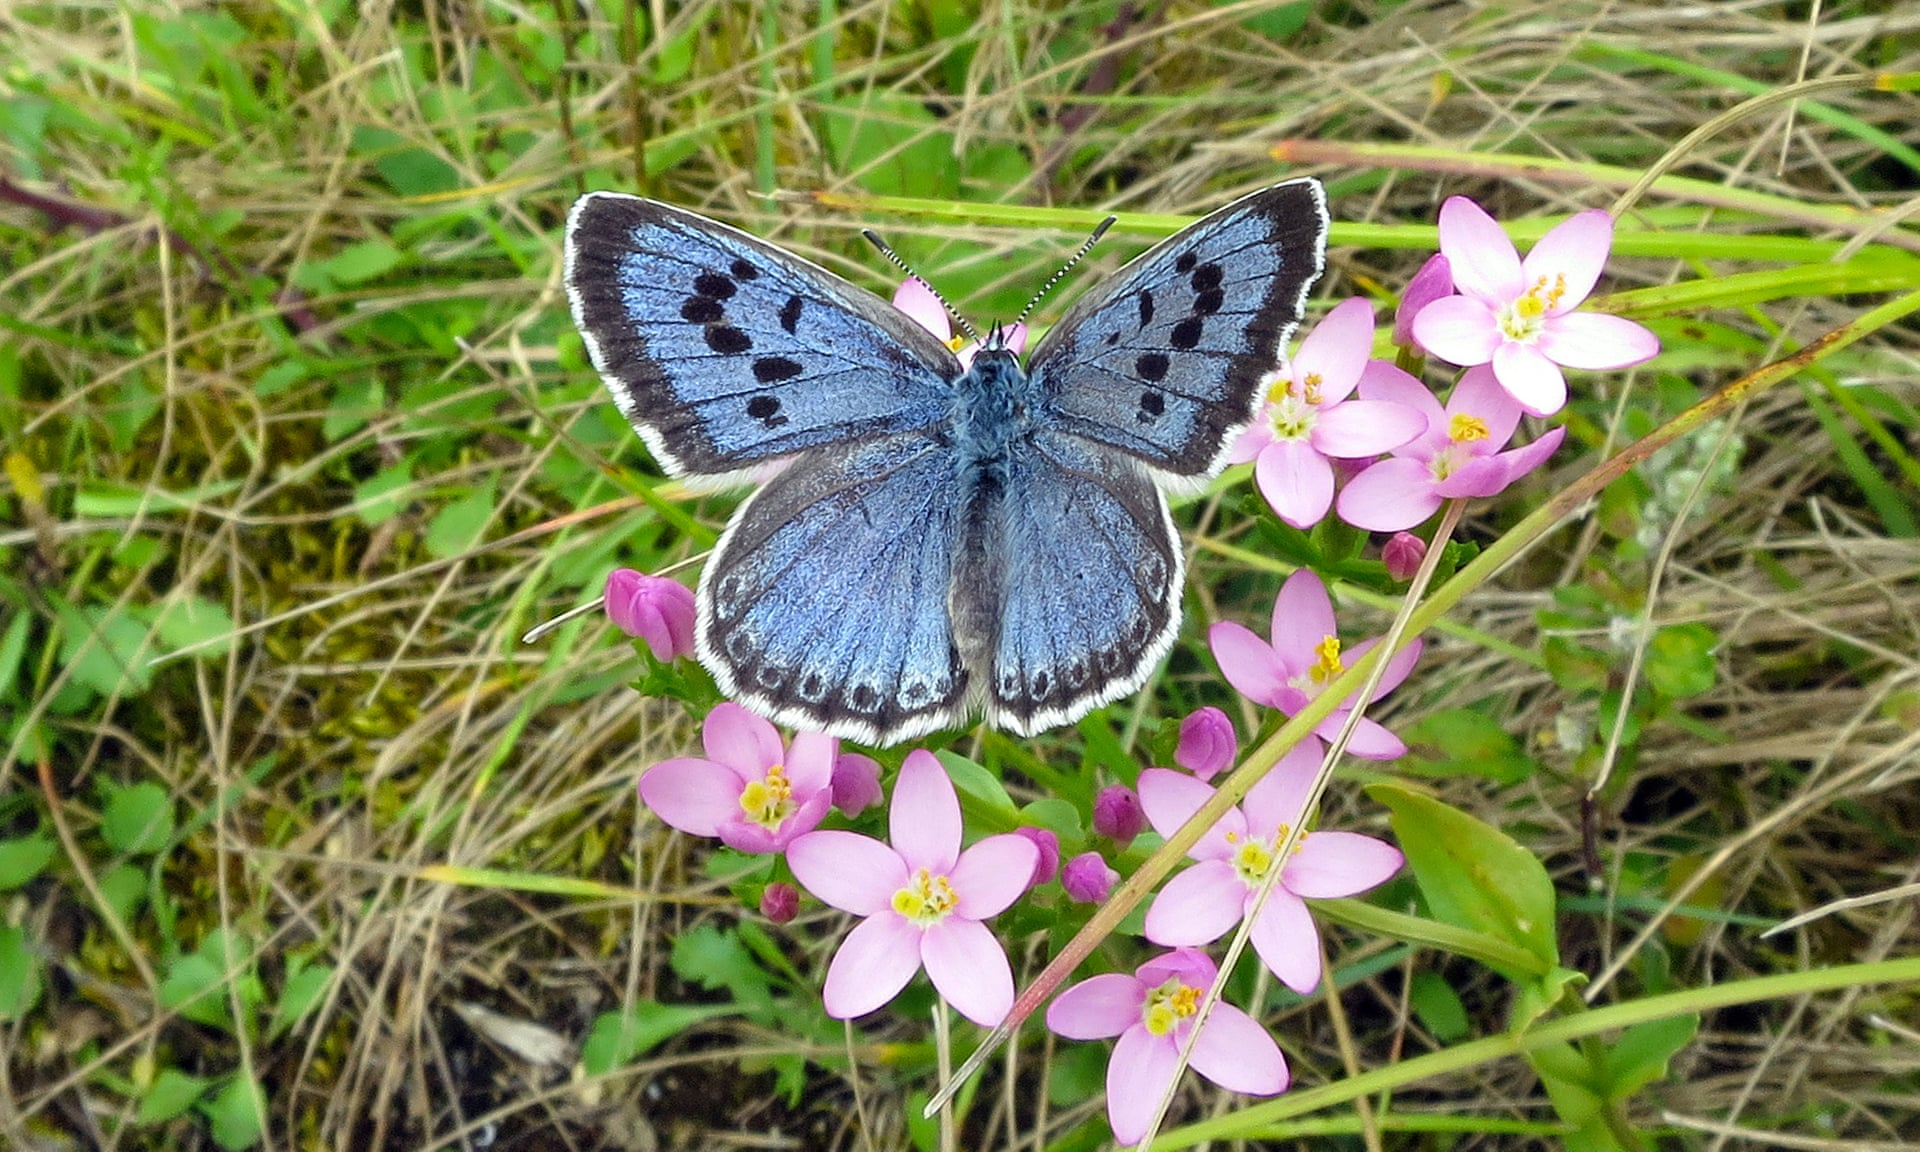
\includegraphics[width=1\columnwidth]{large_blue_1}
	\caption{\textit{M. arion} resting in grassland. Photo taken from \cite{noauthor_large_2018}.} 
	\label{fig:large_blue_1} 
\end{figure}

The life of the large blue is deeply intertwined with its mutualistic partners wild Thyme (\textit{Thymus polytrihcus}) and the red ant (\textit{Myrmica sabuleti}). The large blue selectively lays its eggs on the leaves of wild thyme and after growing into caterpillars, the insects drop to the ground where they infiltrate the nests of \textit{M. sabuleti} \cite{noauthor_expanding_nodate}. Once in these nests, the young caterpillars employ a range of strategies to take advantage of the host ant colony. One such strategy called the "cuckoo" strategy sees \textit{M. arion} caterpillars use acoustic mimicry to play the part of ant larvae in order to coerce food out of their hosts.  

This parasitic, specialist mutualism makes the large blue an interesting subject of scientific inquiry as small changes in its ecosystem have led to drastic declines in population. During the twentieth century the large blue began disappear-- much to the chagrin of scientists whose early attempts at saving the species by targeting butterfly collectors, overgrazing, and air pollution saw little affect. In 1979 the last butterfly in the UK died \cite{noauthor_how_2009}. 

Soon thereafter, efforts to explain the loss of this species increased. Jeremy Thomas, David Simcox, Ralph Clarke identified factors contributing to the decline after performing a careful scientific analysis and comparing to similar populations in Europe \cite{noauthor_how_2009}. The identification of these factors has enabled the steady reintroduction of the species to small areas of the UK with great attention to cultivating the land and resources necessary for this species to survive. As of September 2018, reintroduction sites have had great success! For example, the Polden Hills project, which manages nearly 80\% of the recovering population, has planted 11147 wild thyme plants on 7 sites and manages over 10 hectares of grassland \cite{noauthor_expanding_nodate}. Such efforts have seen led to over 30 successful large blue colonies with as many as 5700 blues being recorded at a single site \cite{noauthor_expanding_nodate, morris_large_2018}. 

The large blue butterfly matters because it is a rare example of a species that has received unilateral conservation efforts from stakeholder groups including scientists, civilians, farmers, the government, and intergovernmental agencies. The successful reintroduction of this species will demonstrate the capacity of humans to cooperate as caretakers of our ecosystems. 

A note of caution though; it is too early to rest on our laurels. Researchers anticipate the recent rises in population will soon decline as drought will cause numbers to drop. The extent to which this unique species is threatened by antrhopogenic climate changes remains to be directly established. Since 1996, the species has maintained a status "nearly threatened" on the IUCN red list \cite{noauthor_iucn_nodate}.

\section*{The Issue/Threat/Problem}

\begin{figure}[!hbt]
	\centering
	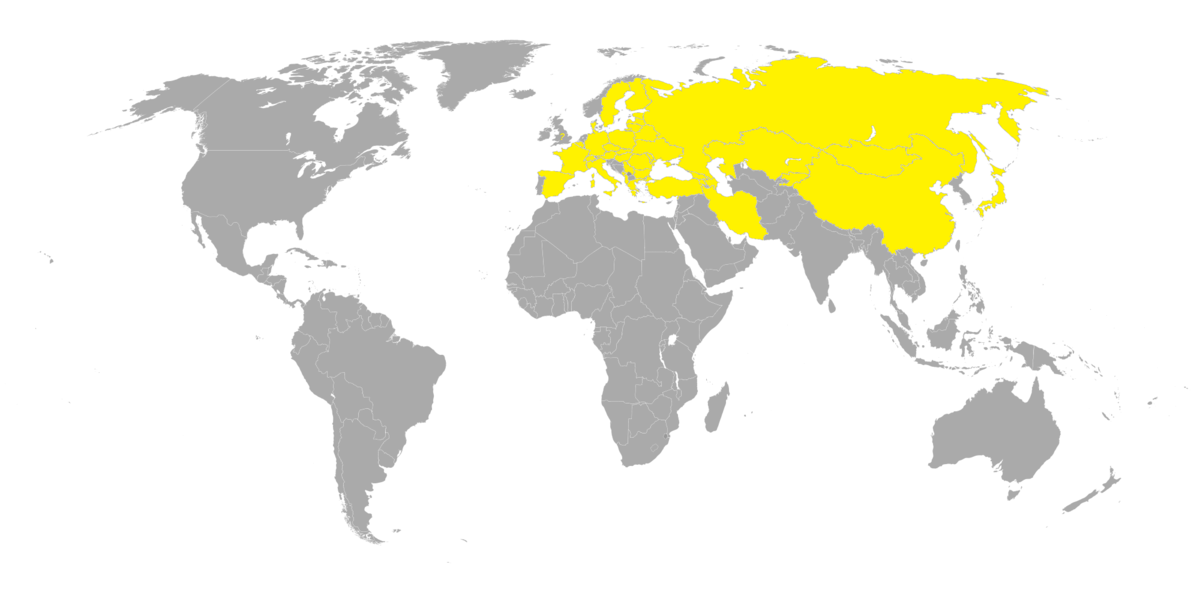
\includegraphics[width=1\columnwidth]{distribution}
	\caption{A map showing the distribution of \textit{M. arion} across the globe. Image taken from \cite{noauthor_large_2018}.} 
	\label{fig:distribution}
\end{figure}

As discussed in the introduction, the large blue butterfly has faced a drastic decline in population including extinction in the United Kingdom. Recent reintroduction of the species has elucidated concerns regarding the following mutualistic / parasitic relationships 
\begin{itemize}
	\item \textit{Myrmica sabuleti}-- the red ant whose colonies the large blue invades as a caterpillar.
	\item \textit{Thymus polytrichus}-- the wild thyme upon which the large blue solely lays its eggs and, by extension, the grasslands where everything resides. 
	\item Species such as rabbits and hares that forage the grasslands to levels that enable the large blue butterfly to survive. 
\end{itemize}

These particular relationships coupled with the changing climate are the key contributors to the decline of the large blue butterfly population and pose significant challenges to their restoration. 

\section*{Solution(s)}  

One of the prime results of research into the life of the large blue butterfly has been the discovery of its close dependence upon state of the grasslands it inhabits. Jeremy Thomas writes that 
\begin{quote}
	"One obvious factor causing the extinction of many Maculinea populations has been the fundamental destruction of their biotopes, for example by drainage, ploughing, the intensification of agriculture and afforestation"
\end{quote}\cite{thomas_ecology_1995}. One reason why this is such a problem is that the ants which the large blue needs to survive rely on the local vegetation maintaining an extremely low height. If vegetation grows too tall (above 1.4cm) then \textit{M. sabuleti}'s brood-chambers become too cool and their numbers fall. Because the large blue's success depends directly on the presence of this species, under-managing these grasslands contributes to butterfly decline \cite{noauthor_how_2009}. 

This example illustrates how further research is needed to identify the interdependencies between butterfly, ant, and environment. Furthermore, once such relationships become known, an education program is necessary in order to make sure that people don't harm a species despite good intentions. The large blue butterfly in particular needs well-drained unimproved grassland- predominantly in limestone or coastal grassland \cite{noauthor_expanding_nodate}. 

Connected to this loss of habitat is the loss of the host ants. In a separate study of large blue populations in France, Thomas concludes that, "the presence of \textit{Myrmica} ant was the crucial factor for large blue populations at each of the sites investigated" \cite{thomas_behaviour_1984}. This strict dependence has led to the conclusion that the narrow niche of \textit{M. arion} makes it difficult to conserve in northern regions with cool climates (like the UK) \cite{thomas_effects_1998}. 

Based off of this evidence, a reasonable solution to the problems facing the large blue butterfly is to direct conservation efforts (and money) towards regions further south in Europe where the climate is warmer and ants are less susceptible to inclement weather. In fact, this opinion is shared by many of the researchers including Thomas who has stated that
\begin{quote}
	"We predict that the conservation of M. arion will be easier and cheaper to achieve under the warm climates of central lowland Europe where different, less intensive, management is required."
\end{quote}  
 \cite{thomas_effects_1998}. I suspect discussion of such an option would be challenging as there has already been significant investment into reintroducing the species to the UK. However, the reality may be that \textit{M. arion} has a better chance of surviving in a different location and, changes in climate will only serve to exacerbate the problem as we will soon discuss. 
 
 So far we have established that large blue butterfly decline is a result of losses to the \textit{Myrmica} ant colonies which, in turn, have suffered due to changes in their grassland ecosystem. Aside from mismanagement of the land, part of the reason for these changes is that grazing mammal populations such as hares and rabbits have suffered simultaneous losses and could therefore not eat enough grasses to maintain the necessary $<3$ cm for ant colonies to thrive. Myxomatosis, a viral disease fatal to rabbits, was introduced in the 1970's and killed off a large percentage of the population that grazed the turf where the ants live \cite{noauthor_how_2009}. 
 
 ... I will continue to talk about grazing mammals and then will make predictions about the possible effects of climate change... 

\section*{Stakeholders/Responsible Parties}
The large blue, 
thyme and other pollinated plants, 
citizens, 
scientists / government (an example of a decisive conservation effort) 
\section*{Global Context} 
	
\bibliography{references}
\bibliographystyle{plain}

\end{document}
